\chapter{Marco teórico}\label{chapter:state-of-the-art}

En este capítulo se presentan los fundamentos teóricos necesarios para el desarrollo de esta investigación. Se abordan los principios del procesamiento digital de imágenes, con especial énfasis en las características y particularidades de las imágenes obtenidas por tomografía computarizada (TC) de cráneo. Asimismo, se describen las técnicas convencionales y actuales de mejora de contraste en imágenes médicas, destacando sus ventajas y limitaciones. Finalmente, se introduce el marco conceptual de la transformada synchrosqueezed, que servirá de base para la propuesta metodológica de mejoramiento de contraste desarrollada en este trabajo.

\section{Representación de imágenes de CT}

En el contexto de esta tesis, una imagen digital se representa formalmente como una matriz $ M \in \mathbb{R}^{n \times m} $, donde cada elemento $ (i, j) $ corresponde a la intensidad o luminancia del píxel ubicado en la fila $ i $ y columna $ j $. En imágenes a color, la representación suele involucrar tres matrices independientes, cada una asociada a la intensidad de los canales rojo, verde y azul (RGB por sus siglas en inglés). Sin embargo, dado que las imágenes de CT son inherentemente monocromáticas, una sola matriz es suficiente para describir la distribución de intensidades, lo que simplifica su procesamiento y análisis.%todo: poner ref 

En el caso particular de las imágenes médicas obtenidas mediante tomografía computarizada de cráneo, cada valor de la matriz representa la atenuación de los rayos X en una región específica del tejido, cuantificada mediante unidades Hounsfield (HU, por sus siglas en inglés). Estas unidades permiten distinguir entre diferentes tipos de tejidos, como hueso, sustancia gris, sustancia blanca y líquido cefalorraquídeo, en función de sus propiedades de absorción.%todo: poner ref

Durante la adquisición de imágenes de tomografía computarizada (CT), se utiliza un equipo especializado compuesto por un escáner de gran tamaño con forma de anillo, denominado gantry. El paciente se recuesta sobre una mesa motorizada que se desplaza lentamente a través del gantry, mientras un tubo de rayos X y un conjunto de detectores electrónicos rotan alrededor de la cabeza del paciente. Este sistema emite haces de rayos X que atraviesan los tejidos y son atenuados en función de sus propiedades físicas; los detectores captan la radiación remanente y envían la información a una computadora central.%todo: poner ref

La computadora procesa los datos recolectados durante las múltiples rotaciones y posiciones del tubo de rayos X, aplicando algoritmos matemáticos avanzados para reconstruir imágenes transversales o cortes bidimensionales del cráneo. Estas imágenes pueden ser posteriormente apiladas para obtener representaciones tridimensionales detalladas, lo que facilita la identificación precisa de estructuras anatómicas y posibles patologías.%todo: poner ref

En el desarrollo de esta tesis, las imágenes médicas utilizadas se almacenan y procesan en el formato NIfTI (Neuroimaging Informatics Technology Initiative, con extensión de archivo \texttt{.nii}). Este formato fue diseñado específicamente para aplicaciones de neuroimagen, superando las limitaciones de formatos previos como Analyze y permitiendo el manejo eficiente de datos multidimensionales, como los obtenidos en estudios de tomografía computarizada (CT) de cráneo. NIfTI posibilita la representación de volúmenes completos, integrando en un solo archivo tanto la información de los datos de imagen como los metadatos relevantes para el análisis, como la orientación espacial y las dimensiones físicas de los vóxeles. Esta capacidad lo convierte en un estándar ampliamente adoptado en la investigación y el procesamiento avanzado de imágenes cerebrales, facilitando la interoperabilidad con herramientas especializadas de análisis y visualización.%todo: poner ref

NIfTI resuelve limitaciones importantes relacionadas con la representación de datos, como la incapacidad de manejar ciertos tipos de datos (por ejemplo, enteros sin signo de 16 bits) y la falta de información precisa sobre la orientación espacial de las imágenes. NIfTI permite almacenar tanto los datos de imagen como los metadatos relevantes en un único archivo o en archivos separados, facilitando la interoperabilidad entre diferentes plataformas y herramientas de análisis . Además, ofrece soporte nativo para imágenes multidimensionales, donde las tres primeras dimensiones corresponden a las coordenadas espaciales $ (x, y, z) $ y la cuarta puede ser utilizada para representar series temporales o parámetros adicionales, lo que resulta especialmente útil en estudios volumétricos y funcionales.

Entre las principales ventajas del formato NIfTI destaca su capacidad para asociar las coordenadas de la imagen con posiciones en el espacio real, mejorando la precisión en el análisis y la comparación entre distintos estudios. Asimismo, su adopción generalizada en la comunidad científica ha impulsado el desarrollo de herramientas especializadas para su visualización y procesamiento, facilitando la reproducibilidad y el intercambio de datos. En el contexto de esta tesis, se emplea un conjunto de datos proveniente de PhysioNet, denominado \emph{Computed Tomography Images for Intracranial Hemorrhage Detection and Segmentation} \cite{DatasetPhysionet,DatasetOriginalArticle}, el cual está disponible en formato NIfTI y proporciona imágenes de tomografía computarizada de cráneo adecuadas para la investigación y validación de técnicas de mejoramiento de contraste.

\section{Aspectos de procesamiento de imágenes}

\subsection{Parámetros fundamentales de la calidad de imagen}

Las imágenes médicas digitales presentan una serie de parámetros fundamentales que determinan su calidad y utilidad diagnóstica. Entre estos parámetros se encuentran el contraste, la resolución espacial, la nitidez y el nivel de ruido, los cuales influyen directamente en la percepción visual de las estructuras anatómicas y en la capacidad de los especialistas para identificar hallazgos relevantes. En esta subsección se describirán brevemente estos parámetros, así como su manifestación visual en las imágenes, proporcionando el marco necesario para comprender los procesos de mejoramiento y análisis aplicados en el procesamiento de imágenes médicas\cite{ImageProcessingBook}.

El contraste se refiere a la diferencia en la intensidad o brillo entre distintas áreas de una imagen, lo que permite distinguir claramente las estructuras anatómicas y detectar posibles anomalías. En el contexto de la tomografía computarizada (CT), el contraste es fundamental para resaltar tejidos con diferentes propiedades de absorción de rayos X, facilitando la identificación de órganos, vasos sanguíneos y lesiones. Para mejorar este contraste, en muchos casos se emplean medios de contraste, que son sustancias químicas administradas al paciente por vía oral, intravenosa o rectal, y que modifican temporalmente la forma en que los rayos X interactúan con los tejidos.

Estos agentes de contraste, como los compuestos yodados en CT, permiten que ciertas áreas del cuerpo absorban más o menos radiación, haciendo que aparezcan más claras u oscuras en la imagen final. De este modo, se mejora la diferenciación entre tejidos normales y patológicos, lo que incrementa la precisión diagnóstica. Aunque el uso de medios de contraste no es obligatorio en todos los estudios, su aplicación es crucial en la evaluación detallada de estructuras específicas y en la detección de lesiones que podrían pasar desapercibidas en imágenes sin contraste. Es importante señalar que, si bien estos medios son generalmente seguros, pueden presentar riesgos mínimos, por lo que su uso debe ser evaluado cuidadosamente por el especialista.

El ruido en las imágenes médicas se manifiesta como variaciones aleatorias e indeseadas en la intensidad de los píxeles, que no corresponden a las características reales de los tejidos o estructuras anatómicas. Este fenómeno puede tener su origen en múltiples factores, como las limitaciones físicas de los detectores, la radiación dispersa, el procesamiento digital y las condiciones de adquisición de la imagen. El ruido degrada la calidad visual, dificultando la identificación de detalles finos y reduciendo la relación señal-ruido, lo que puede comprometer la precisión diagnóstica. En las imágenes de tomografía computarizada, el tipo de ruido más común es el gaussiano, aunque pueden presentarse otras formas dependiendo del equipamiento y el protocolo utilizado. Para mitigar su impacto, se emplean diversas técnicas de reducción de ruido, como el filtrado espacial y métodos avanzados basados en inteligencia artificial, cuyo objetivo es preservar la información relevante sin eliminar detalles críticos para el diagnóstico.

La nitidez, por su parte, se refiere a la claridad con la que se representan los bordes y los detalles en una imagen. Una imagen nítida permite distinguir de manera precisa los límites entre distintas estructuras, lo que facilita la interpretación clínica y la detección de anomalías. La nitidez está directamente relacionada con la resolución espacial del sistema de adquisición y puede verse afectada por factores como el movimiento del paciente, el enfoque del detector y los algoritmos de reconstrucción empleados. Sin embargo, existe una relación inversa entre nitidez y ruido: al aumentar la nitidez, es posible que también se incremente el nivel de ruido, por lo que los sistemas de procesamiento de imágenes deben buscar un equilibrio adecuado entre ambos parámetros para garantizar la mejor calidad diagnóstica posible.

\subsection{Métodos clásicos de mejora de imágenes}

\subsubsection{Filtrado Gaussiano}

El filtrado Gaussiano\cite{GaussianFilter} es una técnica clásica de procesamiento de imágenes utilizada principalmente para la reducción de ruido aleatorio, como el ruido electrónico o de tipo Poisson, en imágenes médicas. Este método se basa en la convolución de la imagen original con una máscara o núcleo Gaussiano, que asigna mayor peso a los píxeles cercanos al centro de la ventana y menor peso a los más alejados. El resultado es un suavizado progresivo de la imagen, que atenúa las fluctuaciones de intensidad no deseadas manteniendo la continuidad de las estructuras anatómicas principales. El filtrado Gaussiano es especialmente útil como etapa de preprocesamiento antes de procedimientos como la segmentación o la visualización, ya que reduce el ruido sin eliminar completamente los bordes relevantes. Sin embargo, su principal limitación radica en la posible pérdida de detalles finos y la leve difuminación de los contornos, lo que requiere un ajuste cuidadoso del parámetro de desviación estándar de la función Gaussiana para equilibrar la reducción de ruido y la preservación de la información estructural.

\begin{figure}[H]
    \centering
    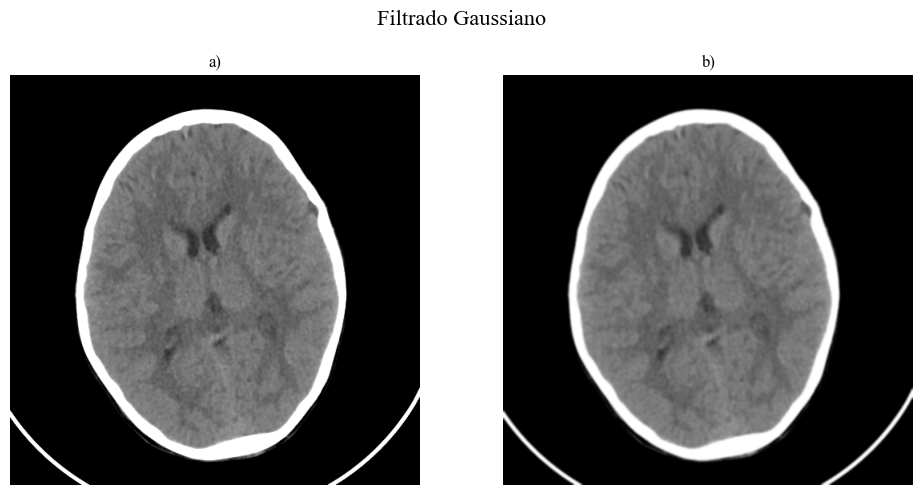
\includegraphics[width=0.95\textwidth]{Graphics/gaussian-filter.png}
    \caption{Comparación visual del efecto del filtrado Gaussiano en una imagen de tomografía computarizada de cráneo: (a) imagen original, (b) imagen tras la aplicación del filtro Gaussiano.}
    \label{fig:filter-gaussian}
\end{figure}

\subsubsection{Filtrado de Mediana}

El filtrado de mediana es otro método ampliamente utilizado para la mejora de imágenes médicas, particularmente eficaz en la eliminación de ruido impulsivo, como el conocido ``ruido sal y pimienta''. A diferencia de los filtros lineales, el filtrado de mediana es un proceso no lineal que reemplaza el valor de cada píxel por la mediana de los valores de intensidad de sus vecinos dentro de una ventana definida. Esta característica permite suprimir eficazmente los valores atípicos sin suavizar excesivamente los bordes ni perder detalles estructurales importantes. Por ello, el filtrado de mediana es especialmente valorado en aplicaciones donde la preservación de las estructuras finas, como vasos sanguíneos o límites tisulares, es prioritaria. No obstante, su desempeño puede verse afectado en presencia de grandes regiones de ruido o cuando se utilizan ventanas demasiado grandes, lo que podría conducir a la pérdida de información relevante\cite{ImageProcessingBook}.

\begin{figure}[H]
    \centering
    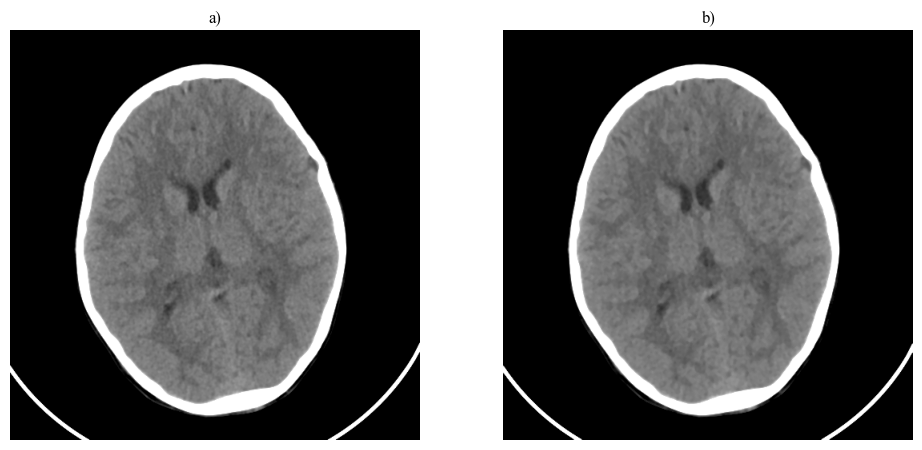
\includegraphics[width=0.95\textwidth]{Graphics/median-filter.png}
    \caption{Comparación visual del efecto del filtrado de mediana en una imagen de tomografía computarizada de cráneo: (a) imagen original, (b) imagen tras la aplicación del filtro de mediana.}
    \label{fig:filter-median}
\end{figure}

\subsubsection{Ecualización Adaptativa del Histograma (CLAHE)}

La ecualización adaptativa del histograma, conocida como CLAHE (Contrast Limited Adaptive Histogram Equalization \cite{CLAHE}), es una técnica avanzada de mejora de contraste que se utiliza ampliamente en el procesamiento de imágenes médicas. A diferencia de la ecualización global de histograma, que redistribuye las intensidades de toda la imagen de manera uniforme, CLAHE divide la imagen en pequeñas regiones o mosaicos y aplica la ecualización de histograma de forma local en cada uno de ellos. Este enfoque permite resaltar detalles en áreas específicas sin amplificar excesivamente el ruido ni crear artefactos indeseados, lo que resulta especialmente útil en imágenes con variaciones locales de contraste, como las obtenidas en tomografía computarizada.

CLAHE incorpora un parámetro de limitación de contraste (\emph{clip limit}) que controla el grado de realce permitido en cada mosaico, evitando la sobre-amplificación del ruido en regiones homogéneas. Además, el tamaño de los mosaicos (\emph{tileGridSize}) puede ajustarse para equilibrar el nivel de detalle local y el efecto global del contraste. Esta técnica ha demostrado ser eficaz para mejorar la visibilidad de estructuras sutiles en tejidos blandos o regiones con bajo contraste, facilitando el análisis y la interpretación clínica. Sin embargo, su aplicación debe realizarse con precaución, ya que un ajuste inadecuado de los parámetros puede introducir artefactos o modificar la apariencia de ciertas regiones relevantes para el diagnóstico.

\begin{figure}[H]
    \centering
    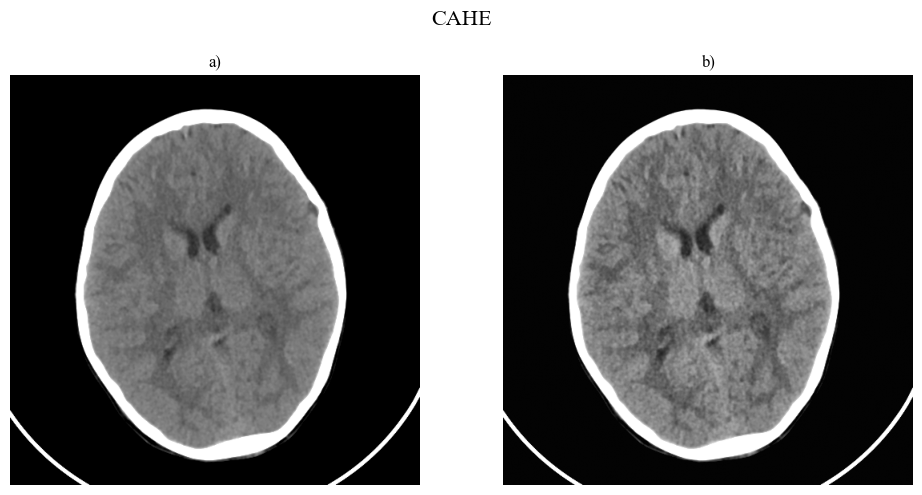
\includegraphics[width=0.95\textwidth]{Graphics/cahe.png}
    \caption{Comparación visual del efecto de la ecualización adaptativa del histograma en una imagen de tomografía computarizada de cráneo: (a) imagen original, (b) imagen tras la aplicación de CLAHE.}
    \label{fig:filter-clahe}
\end{figure}

\subsubsection{Transformación Homomórfica}

La transformación homomórfica \cite{HomomorphicFilter} es un método clásico orientado a la mejora simultánea del contraste y la nitidez en imágenes digitales. Su fundamento radica en el modelado de la imagen como el producto de dos componentes: la iluminación (de baja frecuencia) y la reflectancia (de alta frecuencia). Mediante una transformación logarítmica, este producto se convierte en una suma, permitiendo la aplicación de filtros en el dominio de la frecuencia para atenuar las variaciones lentas de iluminación y realzar los detalles finos asociados a los bordes y texturas.

En el contexto de imágenes médicas, la transformación homomórfica es especialmente útil para corregir problemas de iluminación no uniforme y para destacar estructuras anatómicas que podrían pasar desapercibidas en cortes oscuros o mal iluminados. Tras el procesamiento, se aplica la transformación exponencial inversa para reconstruir la imagen mejorada. Este método ofrece la ventaja de mejorar el contraste local y global de manera simultánea, incrementando la claridad de los bordes y la percepción de detalles relevantes para el diagnóstico. No obstante, la selección adecuada de los parámetros del filtro es crucial para evitar la introducción de artefactos y preservar la información diagnóstica esencial.

\begin{figure}[H]
    \centering
    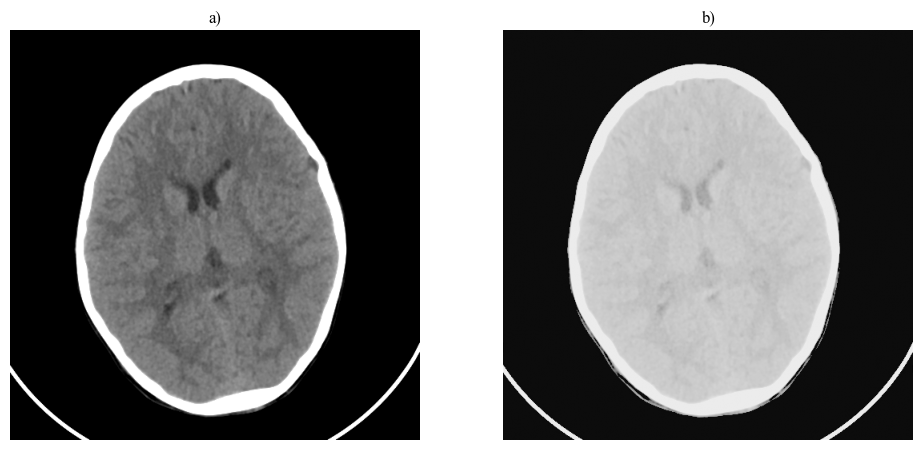
\includegraphics[width=0.95\textwidth]{Graphics/homomorphic.png}
    \caption{Comparación visual del efecto de la transformación homomórfica en una imagen de tomografía computarizada de cráneo: (a) imagen original, (b) imagen tras la aplicación de la transformación homomórfica.}
    \label{fig:filter-homomorphic}
\end{figure}

\subsubsection{Detección de Bordes (Canny o Laplaciano)}

La detección de bordes es una técnica fundamental en el procesamiento de imágenes médicas, cuyo objetivo principal es resaltar los contornos y límites anatómicos presentes en la imagen \cite{CannyBorderDetection,LaplacianBorderDetection}. Los métodos clásicos, como el detector de Canny y el operador Laplaciano, permiten identificar transiciones abruptas de intensidad, que suelen corresponder a los bordes entre diferentes tejidos u órganos. La aplicación de estos algoritmos facilita la delimitación precisa de regiones de interés, como órganos, vasos sanguíneos o lesiones, lo que resulta esencial para tareas posteriores de segmentación, cuantificación y análisis morfológico.

El detector de Canny es especialmente valorado por su capacidad para localizar bordes de forma robusta y continua, minimizando la detección de falsos positivos gracias a su enfoque multietapa que incluye suavizado, cálculo de gradientes, supresión de no-máximos y umbralización con histéresis. Por otro lado, el operador Laplaciano, basado en la segunda derivada de la intensidad, destaca los puntos de cambio rápido en la imagen, aunque es más sensible al ruido y suele emplearse en combinación con técnicas de suavizado previo. En el contexto de la tomografía computarizada, la detección de bordes contribuye significativamente a la mejora de la visualización de estructuras anatómicas y a la precisión de los procesos de diagnóstico asistido por computadora, permitiendo una interpretación más clara y objetiva de las imágenes.

\begin{figure}[H]
    \centering
    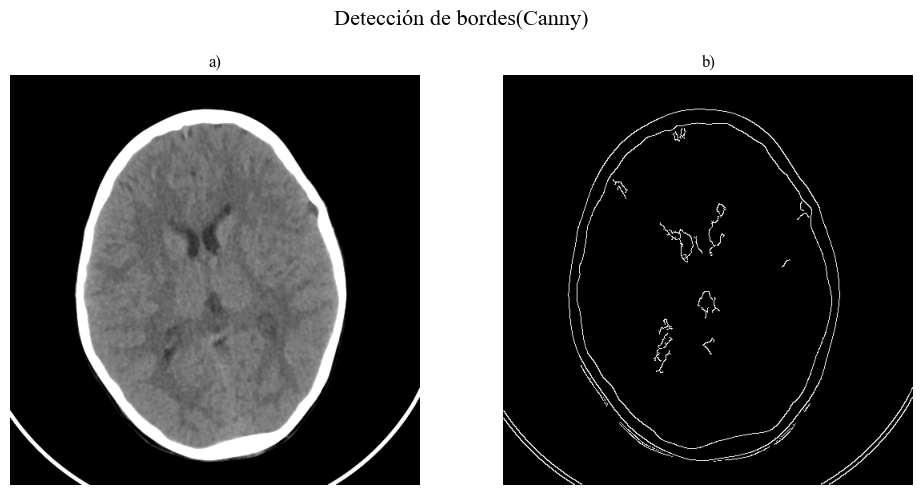
\includegraphics[width=0.95\textwidth]{Graphics/canny.png}
    \caption{Comparación visual del efecto de la detección de bordes mediante el filtro de Canny en una imagen de tomografía computarizada de cráneo: (a) imagen original, (b) imagen tras la aplicación del detector de bordes Canny.}
    \label{fig:filter-canny}
\end{figure}

\subsection{Métodos estado del arte}

\subsubsection{EDCNN}

Uno de los avances recientes en la mejora de imágenes de tomografía computarizada (CT) de baja dosis es el modelo EDCNN (Edge enhancement-based Densely Connected Network \cite{EDCNN}), una red neuronal convolucional diseñada específicamente para la reducción de ruido manteniendo la integridad de los detalles anatómicos. EDCNN introduce un módulo de mejora de bordes que utiliza operadores Sobel entrenables para extraer y realzar características de bordes en múltiples direcciones, integrando estos mapas de bordes con la imagen original como entrada al modelo. Esta estrategia permite preservar estructuras finas y contornos, superando la tendencia al sobresuavizado observada en métodos previos.

La arquitectura de EDCNN se basa en una red completamente convolucional con conexiones densas, inspirada en DenseNet, que facilita la fusión de información jerárquica y de bordes a lo largo de la red. Además, emplea una función de pérdida compuesta que combina el error cuadrático medio (MSE) con una pérdida perceptual multi-escala basada en ResNet-50, lo que favorece la similitud tanto a nivel de píxel como de estructuras visuales. 

Los resultados reportados en el dataset NIH AAPM-Mayo Clinic LDCT demuestran que EDCNN logra una reducción de ruido efectiva y una mejor preservación de detalles en comparación con modelos clásicos y otros métodos de aprendizaje profundo, obteniendo altas puntuaciones en métricas cuantitativas (PSNR, SSIM) y en evaluaciones subjetivas realizadas por radiólogos. Este enfoque representa un avance significativo en el estado del arte para la mejora de imágenes CT de baja dosis, equilibrando la reducción de ruido y la conservación de información diagnóstica relevante.

\subsubsection{LEARN++}

Un avance relevante en el campo de la reconstrucción de imágenes de CT con sensado comprimido es el modelo LEARN++ \cite{LEARN++}. Esta arquitectura, basada en redes neuronales recurrentes de doble dominio, está diseñada para abordar los desafíos asociados a la reconstrucción a partir de un número reducido de vistas y a la reducción de la dosis de radiación. A diferencia de métodos tradicionales y enfoques basados en un solo dominio, LEARN++ procesa simultáneamente la información en los dominios de la imagen y del sinograma, permitiendo una interacción paralela y continua entre ambos. La red integra una subred convolucional dedicada a la restauración de imágenes y otra orientada al "inpainting" adaptativo de sinogramas, logrando así una mayor consistencia de datos y una mejor preservación de detalles anatómicos.

La función de pérdida compuesta de LEARN++ combina el error cuadrático medio tanto en el dominio de la imagen como en el sinograma, junto con una pérdida perceptual basada en características extraídas por VGG-19. Esta combinación permite equilibrar la fidelidad de los datos con la calidad visual y estructural de las imágenes reconstruidas. Los resultados obtenidos en el dataset NIH-AAPM-Mayo Clinic LDCT demuestran que LEARN++ supera significativamente a modelos previos en métricas cuantitativas como PSNR y SSIM, así como en evaluaciones subjetivas realizadas por radiólogos, destacándose por su capacidad para eliminar artefactos, reducir el ruido y preservar estructuras de bajo contraste.

En síntesis, LEARN++ representa un avance significativo en la reconstrucción de imágenes CT de baja dosis, estableciendo un marco generalizable que integra el procesamiento dual-domain y una función de pérdida compuesta. Su versatilidad y robustez lo posicionan como una alternativa eficaz tanto en escenarios clínicos con datos limitados como en aplicaciones de reducción de dosis, contribuyendo al desarrollo de técnicas más seguras y precisas en el ámbito de la imagenología médica.

\subsubsection{ULTRA}

El modelo ULTRA \cite{ULTRA} constituye una propuesta avanzada para la reconstrucción de imágenes en tomografía computarizada espectral (TC espectral) mediante aprendizaje profundo. Basado en una arquitectura U-net modificada con conexiones densas y filtros multicanal, ULTRA está diseñado para fusionar información multiescala y mejorar la extracción de características relevantes en imágenes adquiridas a diferentes energías. Entre sus innovaciones destaca la introducción de una función de pérdida generalizada $ L_p^p $, que permite controlar el equilibrio entre suavizado y preservación de bordes, así como una regularización por variación total anisotrópica que aprovecha las correlaciones espaciales y espectrales entre los distintos bins de energía.

Este enfoque aborda eficazmente los retos inherentes a la TC espectral, como la baja relación señal-ruido y la presencia de artefactos, superando las limitaciones de los métodos tradicionales basados en variación total o diccionarios tensoriales, que suelen ser computacionalmente costosos y sensibles a la selección de parámetros. ULTRA combina los beneficios del aprendizaje profundo con técnicas de regularización física, logrando una reconstrucción eficiente y precisa, con tiempos de procesamiento comparables a los métodos analíticos convencionales.

Los resultados experimentales, tanto en simulaciones como en estudios preclínicos y con fantomas físicos, demuestran que ULTRA supera a los métodos clásicos y otras redes profundas en métricas cuantitativas y cualitativas, preservando detalles anatómicos y mejorando la descomposición de materiales. Estas características posicionan a ULTRA como una solución robusta y escalable para aplicaciones clínicas futuras en TC espectral, con potencial para extenderse a geometrías tridimensionales y escenarios adversos.

\subsubsection{DLR}

Las técnicas de reconstrucción basadas en aprendizaje profundo (Deep Learning Reconstruction, DLR \cite{DLR}) han emergido como una alternativa avanzada para mejorar la calidad de imagen en angiografías por tomografía computarizada cerebral (CTA), superando las limitaciones de los métodos tradicionales como la retroproyección filtrada (FBP) y la reconstrucción iterativa híbrida (Hybrid IR). DLR utiliza redes neuronales convolucionales entrenadas con imágenes de referencia de alta calidad para diferenciar entre señal anatómica y ruido, permitiendo una reducción significativa del ruido y los artefactos sin sacrificar la resolución espacial ni la textura natural de la imagen.

Estudios recientes han demostrado que DLR no solo mejora métricas objetivas como la relación señal-ruido (SNR) y la relación contraste-ruido (CNR), sino que también incrementa la nitidez de bordes y la visualización de vasos pequeños, aspectos críticos en el diagnóstico de patologías vasculares intracraneales. Además, DLR ofrece tiempos de reconstrucción más rápidos que los métodos iterativos basados en modelos, lo que facilita su integración en la práctica clínica diaria. Algoritmos comerciales como AiCE (Canon) y TrueFidelity™ (GE) ya cuentan con validación clínica y aprobación regulatoria, consolidando el papel del aprendizaje profundo en la reconstrucción de imágenes médicas.

En síntesis, la reconstrucción basada en aprendizaje profundo representa un avance sustancial en la calidad y eficiencia de la CTA cerebral, permitiendo una mejor visualización de estructuras vasculares complejas y una reducción de artefactos, con potencial para optimizar el diagnóstico y tratamiento de enfermedades cerebrovasculares.

\section{Propuesta}

\subsection{Transformada Curvelet}

La transformada curvelet es una técnica de análisis multirresolución diseñada para representar de manera eficiente señales e imágenes con singularidades a lo largo de curvas suaves. A diferencia de la transformada wavelet, que ofrece una representación óptima de singularidades puntuales, la curvelet proporciona una representación \textbf{parsimoniosa} de estructuras curvilíneas y bordes en imágenes, gracias a su capacidad de adaptación direccional y anisotropía controlada\cite{Curvelets2000,FastCurveletTransform}.

\subsubsection{Fundamentos Matemáticos}

En su formulación continua, una curvelet se define como una función de base indexada por tres parámetros: 
\begin{itemize}
    \item \textbf{Escala} (\(j \in \mathbb{N}\)): Controla el tamaño de la curvelet.
    \item \textbf{Orientación} (\(\theta_l \in [0, 2\pi)\)): Determina la dirección principal de la curva.
    \item \textbf{Posición} (\(k \in \mathbb{Z}^2\)): Localiza la curvelet en el espacio.
\end{itemize}

La curvelet madre \(\phi_j(x)\) se dilata, rota y traslada para generar la familia de funciones:
\[
\phi_{j,l,k}(x) = 2^{-3j/4} \phi_j \left( R_{\theta_l}^{-1}(x - x_k^{(j,l)}) \right),
\]
donde \(R_{\theta_l}\) es la matriz de rotación y \(x_k^{(j,l)}\) denota la posición central en la escala \(j\) y orientación \(\theta_l\). En el dominio de Fourier, las curvelets se localizan en regiones \textbf{en forma de cuña}, con soporte anisotrópico que satisface la relación:
\[
\text{Ancho} \sim 2^{-j/2}, \quad \text{Largo} \sim 2^{-j}.
\]

\subsubsection{Transformada Curvelet Discreta}

La implementación discreta se realiza en el dominio de Fourier mediante los siguientes pasos\cite{FastCurveletTransform}:
\begin{enumerate}
    \item Aplicar la transformada de Fourier bidimensional (2D FFT) a la imagen.
    \item Multiplicar el espectro por ventanas angulares \(U_{j,l}(\omega)\) que aíslan bandas de frecuencia y dirección.
    \item Reorganizar (\emph{wrapping}) cada cuña espectral en un rectángulo centrado en el origen.
    \item Aplicar la transformada inversa de Fourier (2D IFFT) para obtener los coeficientes curvelet \(c(j,l,k)\).
\end{enumerate}

Matemáticamente, los coeficientes se calculan como:
\[
c(j,l,k) = \frac{1}{(2\pi)^2} \int_{\mathbb{R}^2} \hat{f}(\omega) U_{j,l}(\omega) e^{i\langle x_k^{(j,l)}, \omega \rangle} d\omega,
\]
donde \(\hat{f}(\omega)\) es el espectro de la imagen original.

\subsubsection{Ventajas sobre Otras Transformadas}

La curvelet supera a la wavelet en dos aspectos clave:
\begin{itemize}
    \item \textbf{Sensibilidad direccional}: Detecta bordes y curvas en múltiples orientaciones.
    \item \textbf{Representación esparsa}: Requiere menos coeficientes para representar edges, reduciendo redundancia.
\end{itemize}

Estas propiedades la hacen ideal para aplicaciones en imágenes médicas, donde la preservación de bordes anatómicos y la supresión de ruido son críticas.

\subsection{Transformada Synchrosqueezed Curvelet}

La transformada Synchrosqueezed Curvelet (SSCT) es una técnica avanzada de post-procesamiento que combina la capacidad direccional de la transformada curvelet con un método de reasignación espectral para lograr una representación más precisa de componentes modales en imágenes. Este enfoque es particularmente efectivo para analizar señales bidimensionales con frentes de onda curvos o componentes de banda estrecha, donde los métodos tradicionales fallan en separar modos superpuestos\cite{SynchrosqueezedCurveletTransform}.

\subsubsection{Principios Fundamentales}

La SSCT opera en dos etapas principales:
\begin{enumerate}
    \item \textbf{Transformada Curvelet Generalizada}: Aplica una transformada curvelet con parámetros de escalado geométrico adaptativos (escala radial \(t\) y angular \(s\)) para capturar componentes direccionales.
    \item \textbf{Reasignación Espectral (Synchrosqueezing)}: Reubica los coeficientes curvelet en el espacio fase basándose en estimaciones precisas de vectores de onda locales, condensando la energía en regiones más compactas.
\end{enumerate}

\subsubsection{Formulación Matemática}

Dada una imagen \(f(x)\), la SSCT se define mediante:
\begin{itemize}
    \item \textbf{Transformada Curvelet}: 
    \[
    W_f(a, \theta, b) = \langle f, \phi_{a,\theta,b} \rangle = \int_{\mathbb{R}^2} f(x) \overline{\phi_{a,\theta,b}(x)} dx
    \]
    donde \(\phi_{a,\theta,b}(x)\) son las curvelets con escala \(a\), orientación \(\theta\), y posición \(b\).
    
    \item \textbf{Estimación del Vector de Onda Local}:
    \[
    v_f(a, \theta, b) = \frac{\nabla_b \arg(W_f(a, \theta, b))}{2\pi}
    \]
    Este operador de fase estima la frecuencia instantánea en la dirección dominante.
    
    \item \textbf{Reasignación}:
    Los coeficientes se reubican según:
    \[
    T_f(v, b) = \int_{A(v, b)} W_f(a, \theta, b) a^{-3/2} da d\theta
    \]
    donde \(A(v, b) = \{(a, \theta): v_f(a, \theta, b) = v\}\) agrupa coeficientes con el mismo vector de onda estimado\cite{SynchrosqueezedCurveletTransform}.
\end{itemize}

\subsubsection{Ventajas Clave}

\begin{itemize}
    \item \textbf{Resolución Mejorada}: El synchrosqueezing reduce la dispersión espectral de los coeficientes curvelet, produciendo representaciones más nítidas (Fig. 2).
    \item \textbf{Separación de Modos}: Para señales \(f(x) = \sum_k f_k(x)\) con vectores de onda bien separados (\(|\nabla \phi_k - \nabla \phi_l| \geq d\)), la SSCT identifica cada componente \(f_k\) mediante clustering en el espacio fase reasignado.
    \item \textbf{Invariancia a la Curvatura}: A diferencia de métodos basados en wavelets, preserva la estructura de componentes curvilíneos gracias a la anisotropía de las curvelets.
\end{itemize}

\subsubsection{Aplicación en Procesamiento de Imágenes Médicas}

En el contexto de tomografías de cráneo, la SSCT permite:
\begin{itemize}
    \item Mejorar el contraste mediante la separación espectral de tejidos con diferentes propiedades de atenuación.
    \item Reducir artefactos de "blooming" en estructuras metálicas mediante la reasignación selectiva de coeficientes.
    \item Cuantificar texturas anatómicas mediante el análisis de mapas de vectores de onda locales.
\end{itemize}

\subsection{Propuesta Metodológica}

La propuesta desarrollada en esta tesis consiste en la aplicación de la transformada Synchrosqueezed Curvelet (SSCT) a imágenes de tomografía computarizada (CT) del cerebro. El procedimiento se inicia con la descomposición de la imagen original mediante la SSCT, obteniendo así una representación espectral detallada en el dominio espacio-frecuencia, capaz de capturar tanto las singularidades direccionales como la información multiescala inherente a las estructuras anatómicas cerebrales. Posteriormente, los coeficientes obtenidos a través de la SSCT son modificados mediante una función de procesamiento adecuada, diseñada para realzar las características de interés (como bordes o texturas) o atenuar componentes indeseados (como ruido o artefactos). Finalmente, se reconstruye la imagen a partir de los coeficientes modificados, generando una versión mejorada que se espera presente mayor calidad diagnóstica, con mejor contraste y preservación de detalles relevantes.

Cabe destacar que esta metodología es de naturaleza numérica pura y no depende de técnicas de inteligencia artificial ni de aprendizaje profundo. A diferencia de los métodos basados en redes neuronales, que han demostrado excelentes resultados en la mejora de imágenes médicas pero requieren grandes volúmenes de datos etiquetados, conocimien

\subsubsection{Thresholding}

El método de thresholding consiste en aplicar un umbral fijo a la energía obtenida por la SSCT, de modo que sólo se conserven los valores superiores a un cierto nivel predefinido. Este procedimiento es ampliamente utilizado en el procesamiento de imágenes médicas para segmentar regiones de interés o eliminar componentes de bajo valor energético, facilitando la extracción de estructuras relevantes \cite{zhao2023thresholding, pmc6132127}. La elección del valor de umbral es un parámetro crítico, ya que determina el equilibrio entre la preservación de detalles y la supresión de ruido o artefactos.

\subsubsection{Potenciación de la Energía SSCT}

La potenciación de la energía SSCT consiste en modificar los valores obtenidos de la transformada elevando la energía a una potencia específica (parámetro de enhancement). Esta operación no lineal permite realzar selectivamente las diferencias entre regiones de alta y baja energía, incrementando el contraste local y facilitando la discriminación de estructuras anatómicas sutiles. Métodos de potenciación y manipulación no lineal de coeficientes han sido explorados en el contexto de transformadas multiescala para el realce de imágenes médicas, mostrando mejoras en la percepción visual y en métricas objetivas de calidad \cite{SynchrosqueezedCurveletTransform, EnergyEnhancement}.

\subsubsection{Enmascaramiento del Resultado de la Transformada SSCT}

El enmascaramiento consiste en aplicar una máscara binaria o ponderada sobre el dominio SSCT, permitiendo conservar únicamente aquellas regiones que cumplen ciertos criterios (por ejemplo, localización anatómica, dirección predominante o magnitud de energía). Esta técnica es útil para focalizar el procesamiento en áreas de interés clínico y reducir la influencia de regiones irrelevantes o ruidosas. El enmascaramiento en el dominio de transformadas ha sido utilizado para mejorar la segmentación y el análisis de imágenes médicas, optimizando la relación señal-ruido y la especificidad de los resultados \cite{SynchrosqueezedCurveletTransform,ImageMaskingBook}.to experto para la curación de los conjuntos de entrenamiento y recursos computacionales avanzados (como procesadores gráficos de alto rendimiento), la propuesta aquí presentada puede implementarse con recursos computacionales convencionales y sin la necesidad de datos adicionales. Esta característica resulta especialmente ventajosa en contextos como el cubano, donde el acceso a infraestructuras de cómputo especializadas y bases de datos extensas es limitado.

\vspace{0.5cm}

En síntesis, la propuesta metodológica se fundamenta en el uso de herramientas matemáticas robustas y eficientes para el procesamiento de imágenes médicas, ofreciendo una alternativa viable y accesible para la mejora de la calidad de imágenes de CT cerebral en entornos con restricciones tecnológicas y de recursos humanos.
